\hypertarget{lecture-9-notes}{%
\section{Lecture 9 notes}\label{lecture-9-notes}}

\hypertarget{professor-prof.-lalitha-vadlamani}{%
\subsection{Professor: Prof.~Lalitha
Vadlamani}\label{professor-prof.-lalitha-vadlamani}}

\hypertarget{authors-ananya-sane-l-lakshmanan}{%
\subsection{Authors: Ananya Sane, L
Lakshmanan}\label{authors-ananya-sane-l-lakshmanan}}

\begin{center}\rule{0.5\linewidth}{0.5pt}\end{center}

\hypertarget{key-ideas}{%
\subsection{Key Ideas}\label{key-ideas}}

\begin{enumerate}
\def\labelenumi{\arabic{enumi}.}
\item
  Lemmas for the CDF
\item
  Types of random variables
\end{enumerate}

\begin{center}\rule{0.5\linewidth}{0.5pt}\end{center}

\textbf{Lemma :} For any \(x \in R\)

\(P(X = x) = P(X \leq x) - P(X < x)\)

Then, by continuity of probability,

\(P(X = x) = F_X(x) - \displaystyle\lim_{\epsilon \to 0} F_X(x -\epsilon)\)

\textbf{Corollary :} \(F_X()\) is left continuous iff
\(P(X = x) = 0 \ \ \forall \ \ x \in R\)

This implies \(F_X()\) is continuous iff
\(P(X = x) = 0 \ \ \forall \ \ x \in R\)

\hypertarget{types-of-random-variables}{%
\subsubsection{Types of random
variables}\label{types-of-random-variables}}

\begin{itemize}
\item
  Continuous Random Variable
\item
  Discrete Random Variable
\item
  Mixed Random Variable

  \textbf{(Not done in class)} There is a fourth type of random variable
  called a SINGULAR random variable, that is a fundamentally different
  random variable. It is mostly only of academic interest as it does not
  have many applications. Any probability measure on the Real numbers
  can be broken down into these three fundamental components, i.e.,
  Discrete, Continuous and singular.
\end{itemize}

\hypertarget{continuous-random-variables}{%
\paragraph{Continuous Random
variables}\label{continuous-random-variables}}

A random variable X with CDF \(F_X()\) is said to be continuous if
\(F_X()\) is continuous. In the context of continuous RVs, probabilities
of intervals give useful info, as probabilities of points are always 0.

If \(F_X()\) is a differentiable function, then we can find another
function for the continuous RV, which is defined as,
\[f_X(x) = \frac{dF_X(x)}{dx}\]

which is called the \textbf{probability density function}. We can
integrate this function from \(-\infty\) to whatever value we want to
get the CDF.

So we can say that
\(P(a \leq x \leq b) = \displaystyle\int_{a}^{b}f_X(x)\cdot dx\)

And from this, if we find \(P(x \leq X \leq x + \Delta x)\) and make
\(\Delta x \to 0\), we can approximate it to a rectangle with area
\(f_X(x) \cdot \Delta x\).

\begin{figure}
\centering
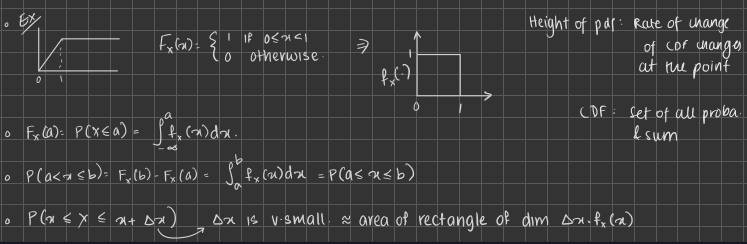
\includegraphics{Screenshot_from_2021-08-07_11-45-20.png}
\caption{Example}
\end{figure}

Properties of a PDF

\begin{itemize}
\tightlist
\item
  \(f_X(x) \geq 0\) (Because CDF is monotonically non decreasing)
\item
  \(\displaystyle\int_{-\infty}^{\infty}f_X(x)\cdot dx = 1\)
\end{itemize}

\emph{PDF by itself does not indicate any probability.}

\hypertarget{radon-nikodyn-theorem-not-done-in-class}{%
\paragraph{Radon Nikodyn theorem (Not done in
class)}\label{radon-nikodyn-theorem-not-done-in-class}}

Let X be a continuous RV. There exists a non negative measurable
function \(f_x() : R \to [0, \infty)\) such that for any B in the Borel
sigma algebra, we have

\[P_X(B) = \displaystyle\int_{B} f_x\cdot d\lambda\]

This basically means for any Borel set, we can represent its probability
law as the integral of a non negative function. As we have not done
measure theory yet, we can understand it as an integration over the real
line for our purposes. This is the basis for the equation that relates
the CDF of continuous random variables to the PDF, i.e.,

\[P_X((-\infty, x]) = F_X(x) = \displaystyle\int_{-\infty}^{x} f_X(x) dx\]

\hypertarget{discrete-random-variables}{%
\paragraph{Discrete Random Variables}\label{discrete-random-variables}}

X is said to be a discrete random variable if the range of X is either
finite or countably infinite in R.

The CDF of a discrete random variable will look like a staircase,
constant everywhere, with jumps at certain points.

Here, \(P(X = x_i) > 0\), not necessarily, but possible. CDF for this
would be

\[F_X(a) = \displaystyle\sum_{x_i \leq a} P(X = x_i)\]

Now, \(P(X = x_i) = P_X(x_i)\) for \(x_i\) in the range of X.

\(P_X()\) is called the \textbf{probability mass function}.

Properties of PMF:

\begin{itemize}
\tightlist
\item
  \(P_X(x_i) \geq 0\)
\end{itemize}

For S = range of X = \(\{x_1, x_2, ...\}\)

\begin{itemize}
\tightlist
\item
  \(\displaystyle\sum_{x_i \in S} P_X(x_i) = 1\)
\end{itemize}

\begin{center}\rule{0.5\linewidth}{0.5pt}\end{center}
